% ----------------------------------------------------------
\chapter{Modelo mecânico}
\label{cap: modelo mecanico}
% ----------------------------------------------------------

Esse capítulo traz uma descrição geral do modelo mecânico que será utilizado neste trabalho. Portanto, são apresentadas as equações de equilíbrio e constitutivas que foram utilizadas, sem aprofundar, no entanto, nas particularidades que compreendem o domínio de um túnel profundo. Essas serão vistas no final do Capitulo 6, após a descrição da solução desse modelo mecânico. 

\section{Equações de Equilíbrio local e a hipótese da evolução quase estática}

Sendo $\left\{\underline{e}_1,\underline{e}_2,\underline{e}_3\right\}$ a base de um espaço $\mathbb{R}^3$, a segunda lei fundamental do equilíbrio dinâmico, ou seja, o princípio da conservação do momento linear, aplicada sobre um subdomínio contínuo $\Omega'$, exige que para $\forall \Omega' \subset \Omega$:
\begin{equation}
	\label{eq:conservacao_momento_linear}
\int_{\Omega'}\rho(\gammal-\fl)d\Omega' = \int_{\partial\Omega'}\Tl dS
\end{equation}
sendo $\rho$ a densidade do domínio, $\gammal$ o campo de acelerações referente às forças inerciais, $\fl$ o campo de acelerações referente às forças de corpo (por exemplo, a gravidade) e $\Tl$ o vetor tensão que atua na superfície $dS$ contida na superfície $\partial\Omega'$ de $\Omega'$ (\autoref{subsistema_material}).

\begin{figure}[H]
	\begin{center}
		\includegraphics[scale = 1.0]{0501-subsistema no sistema material forças de corpo.pdf}
	\end{center}
	\caption{\label{subsistema_material}Subsistema material $\Omega'$ no interior de um sistema material $\Omega$ submetido a um campo de forças de corpo}
\end{figure}

Considerando a definição $\Tl = \sigmall \cdot \nl$ , em que $\nl$ é o vetor normal à superfície $dS$ e $\sigmall$ o tensor de tensões, aplicando o teorema da divergência no termo à direita da igualdade (\ref{eq:conservacao_momento_linear}) pode-se escrever que
\begin{equation}
	\label{teorema_divergencia}
	\forall \Omega' \subset \Omega ~~~~ \int_{\Omega'}\left( \divl \sigmall+ \rho(\gammal-\fl) \right)d\Omega' = \underline 0
\end{equation}
e, portanto,
\begin{equation}
	\label{eq:resultado_teorema_divergencia}
	 \underline \nabla \cdot \underline{\underline\sigma}+ \rho(\underline\gamma-\underline f) = \underline 0
\end{equation}
em que $\divl$ é o operador divergente. Aplicando a hipótese de evolução quase estática, ou seja, $\gammal = \underline 0$, tem-se o seguinte sistema de equações de equilíbrio estático local:
\begin{equation}
	\label{eq:equilibrio_estatico_local}
	\divl \sigmall+ \rho \fl = \underline 0.
\end{equation}

Salienta-se também que pela conservação do momento angular tem-se que o tensor de tensões é simétrico, ou seja, $\sigmall = \sigmall^T$ e o sistema (\ref{eq:equilibrio_estatico_local}), em três dimensões, possui 3 equações e 6 incógnitas de tensões.

\section{Admissibilidade estática, natureza Euleriana do Campo de Tensões, Transformação geométrica e medida de deformação}

Para que o sistema material $\Omega$ da \autoref{sistema_material_contorno} esteja em equilíbrio, ou seja, \textbf{estáticamente admissível (E.A)}, o campo de tensões deve satisfazer as equações de campo de equilíbrio local, conjuntamente com as condições de continuidade interna e de contorno (relativo ao princípio da ação-reação) representadas por (\ref{eq:EA}).

\begin{figure}[H]
	\begin{center}
		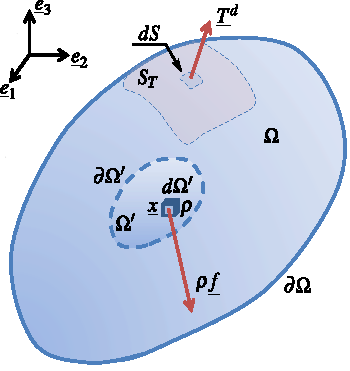
\includegraphics[scale = 1.0]{0502-sistema material com condição de contorno.pdf}
	\end{center}
	\caption{\label{sistema_material_contorno}Sistema material $\Omega'$ com condição de contorno $\underline T^d$ imposta na fronteira $S_T$}
\end{figure}

\begin{equation}
	\label{eq:EA}
	\sigmall~~ \text{é E.A.} \leftrightarrow \left\{
		\begin{matrix}
			\text{eqs. campo:} \left\{
				\begin{matrix}
					\divl \sigmall+ \rho \fl = \underline 0 \\ 
					\sigmall \cdot \nl ~~ \text{contínuo ao longo de} ~~ \Sigma
		
				\end{matrix}\right. \\ 
			\text{cond. contorno:}~~ \sigmall \cdot \nl = \Tl^d ~~ \text{em} ~~ \forall \xl \in S_T \subset \partial \Omega
		\end{matrix}\right.,
\end{equation}

em que $\Sigma$  representa as superfícies de descontinuidades de $\sigmall$ no interior do corpo, se houver. A rigor o campo de tensões $\sigmall$ que satisfaz (\ref{eq:EA}) se refere sempre à configuração atual durante a evolução do sistema, ou seja, possui uma natureza Euleriana (conforme \autoref{tensoes_Euleriana}).

\begin{figure}[H]
	\begin{center}
		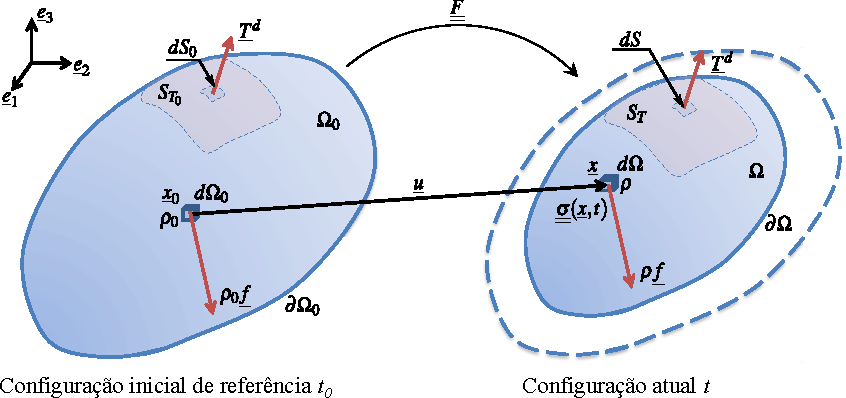
\includegraphics[scale = 1.0]{0503-descricao euleriana do campo de tensoes.pdf}
	\end{center}
	\caption{\label{tensoes_Euleriana}Natureza Euleriana do campo de tensões}
\end{figure}

O vetor $\ul = \xl - \xl_0$ é o deslocamento da partícula durante a evolução do sistema e $\Fll$ é o gradiente da transformação geométrica que associa a posição de cada partícula $\xl_0$ a sua posição $\xl$ na configuração atual, definido por:
\begin{equation}
	\label{eq:transformacao_geometrica}
 	\Fll = \nabla \xl = \nabla \left( \xl_0+\ul \right) = \Umll + \nabla \ul
\end{equation}
em que $\nabla$ é o operador gradiente e $\Umll$ o tensor de segunda ordem unitário. Nesse contexto geral, a medida de deformação mais comum é dada pelo desvio da transformação em relação à isometria $\Fll^T \cdot \Fll = \Umll$ e é descrita através do tensor de deformações de Green-Lagrange:
\begin{equation}
	\label{eq:green_lagrange}
	\greenll = \frac{1}{2} \left(\Fll^T \cdot \Fll - \Umll \right) = \frac{1}{2} \left(\nabla \ul + \nabla\ul^T + \nabla\ul^T \cdot \nabla \ul \right).
\end{equation}

Em problemas quase-estáticos isotérmicos, quando os deslocamentos, as deformações e as rotações são pequenas, a determinação dos campos de tensões e deformações durante a evolução do sistema pode ser simplificada descrevendo os elementos da admissibilidade estática (\ref{eq:EA}) em termos da configuração de referência ao invés da atual. Para tanto, é necessário verificar-se a hipótese das pequenas perturbações.

\section{Hipótese das pequenas perturbações e a descrição Lagrangeana}

A \textbf{hipótese das transformações infinitesimais (HTI)} supõe que o gradiente da transformação é aproximadamente a identidade, ou seja, $\Fll \approx \Umll$ . Isso implica, por (\ref{eq:transformacao_geometrica}), que $\left| \nabla \ul \right| \ll 1$ e, como consequência, pode-se desprezar os termos de derivada mais alta no tensor de deformações de Green-Lagrange, de modo que:
\begin{equation}
	\label{eq:green_lagrange_linearizado}
	\greenll = \frac{1}{2} \left(\Fll^T \cdot \Fll - \Umll \right) = \frac{1}{2} \left(\nabla \ul + \nabla\ul^T + \nabla\ul^T \cdot \nabla \ul \right) \approxeq \frac{1}{2} \left(\nabla \ul + \nabla\ul^T \right) = \nabla^s\ul = \varepsilonll
\end{equation}
em que $\varepsilonll$ é um tensor simétrico conhecido como tensor de deformações de Green-Lagrange linearizado, ou simplesmente, como tensor de deformações. Dessa hipótese segue-se também uma simplificação no \textbf{Jacobiano da transformação} (que dá a relação entre o volume infinitesimal da configuração atual e de referência):
\begin{equation}
	\label{eq:jacobiano}
	J = \frac{d\Omega}{d\Omega_0} = \text{det}\left(\Umll + \nabla \ul \right) \approxeq 1 + \text{tr}(\varepsilonll)
\end{equation}
sendo det($*$) e tr($*$) as funções determinante e traço, respectivamente. Como  $\left| \nabla \ul \right| \ll 1$ tem-se também que $\left| \nabla \varepsilonll \right| \ll 1$, ou seja, \textbf{pequenas deformações}, o que implica $\text{tr}(\varepsilonll) \ll 1$ e, portanto, mudanças infinitesimais no volume e na densidade durante a evolução do sistema, fazendo com que $\Omega \approxeq \Omega_0$ e $\rho \approxeq \rho_0$, respectivamente. Supondo que também ocorram \textbf{pequenos deslocamentos} $\left| \ul / l_0 \right| \ll 1$, em que $l_0$ é uma dimensão característica do problema tal que os efeitos sobre os esforços internos devido a mudança de geometria sejam desprezíveis, tem-se a \textbf{hipótese das pequenas perturbações (HPP)}. Com as consequências dessa hipótese, pode-se adotar a configuração inicial (de referência) ao invés da atual para expressar os termos da admissibilidade estática  (\ref{eq:EA}).

\section{Modelo constitutivo elástico}

De uma forma geral, a energia interna específica $w$  necessária para deformar um material elástico não depende do trajeto e nem da velocidade de deformação durante a evolução do sistema, dependendo apenas do estado atual das deformações. Com isso a energia interna específica pode ser caracterizada pelas deformações e direções principais do tensor de deformações, de modo que:
\begin{equation}
	\label{eq:energia_interna_elastica}
	w(\varepsilonll) = w(\varepsilon_1,\varepsilon_2,\varepsilon_3,\eta_1,\eta_2,\eta_3).
\end{equation}

Contudo, na \textbf{elasticidade isótropa} a energia de deformação é independente das direções principais e pode ser descrita em função apenas da magnitude das deformações principais, ou dos invariantes do tensor de deformação, de modo que
\begin{equation}
	\label{eq:energia_interna_elastica_isotropa}
	w(\varepsilonll) = w(\varepsilon_1,\varepsilon_2,\varepsilon_3) = w(I_1,I_2,I_3),
\end{equation}
sendo que os invariantes do tensor de deformações são dados por:
\begin{equation}
	\label{eq:I1}
	I_1 = \text{tr}(\varepsilonll) = \varepsilon_{ii},
\end{equation}
\begin{equation}
	\label{eq:I2}
	I_2 = \text{tr}(\varepsilonll^2) = \frac{1}{2} \varepsilon_{ij} \varepsilon_{ji},
\end{equation}
\begin{equation}
	\label{eq:I3}
	I_3 = \text{tr}(\varepsilonll^3) = \frac{1}{3} \varepsilon_{ij} \varepsilon_{jk} \varepsilon_{ki}.
\end{equation}

A lei do comportamento elástico se obtém de $\sigmall = \partial w / \partial \varepsilonll$ . Aplicando a regra da cadeia em relação aos invariantes e fazendo uma aproximação de primeira ordem em torno de $\sigmall_0$ tem-se a seguinte lei constitutiva da \textbf{elasticidade linear isótropa}
\begin{equation}
	\label{eq:lei_elasticidade}
	\sigmall - \sigmall_0 = \Dllll:\varepsilonll,
\end{equation}
em que $\Dllll$ é o tensor constitutivo elástico de quarta ordem simétrico dado por
\begin{equation}
	\label{eq:tensor_constitutivo_elastico}
 	\Dllll = \lambda^e \Umll \otimes \Umll + 2 \mu^e \Umllll
\end{equation}
sendo $\underline{\underline 1} \otimes \underline{\underline 1}$ o tensor de quarta ordem dado pelo produto tensorial ($\otimes$) entre dois tensores unitários de segunda ordem e $\underline{\underline{\underline{\underline 1}}}$ o tensor unitário de quarta ordem. As constantes $\lambda^e$ e $\mu^e$ são conhecidos como os coeficientes de Lamè, que possuem as seguintes relações com o módulo de Young $E$ e o coeficiente de Poisson $\nu$:
\begin{equation}
	\label{eq:lambdae}
	\lambda^e = \frac{E \nu}{(1+\nu)(1-2\nu)},
\end{equation}
\begin{equation}
	\label{eq:mue}
	\mu^e = \frac{E}{2(1+\nu)}.
\end{equation}

\section{Modelo constitutivo elastoplástico}

Para problemas com evolução isotérmica, quase-estáticos em transformações infinitesimais, o modelo constitutivo elastoplástico pode ser completamente descrito através da:
\begin{alineas}
	\item decomposição do tensor de deformação total;
	\item superfície de escoamento;
	\item regra de fluxo plástico;
	\item lei de endurecimento/amolecimento;
	\item condições de carregamento/descarregamento.
\end{alineas}

\subsection{Decomposição do tensor de deformação total}
Considerando a hipótese das pequenas transformações (que inclui a hipótese das pequenas deformações) é válida a decomposição do tensor de deformação total em uma componente elástica e outra plástica, de modo que:
\begin{equation}
	\label{eq:decomposicao_deformacoes}
	\dot \varepsilonll = \dot \varepsilonll^e + \dot \varepsilonll^p 
\end{equation}
sendo $\dot \varepsilonll^e$ e $\dot \varepsilonll^p$ as taxas de deformação elástica e plástica, respectivamente. A taxa de deformação plástica também é conhecida por fluxo plástico. Diferentemente do modelo elástico, o modelo elastoplástico é dependente do trajeto das tensões e por isso (\ref{eq:decomposicao_deformacoes}) é descrito em forma de taxas. No entanto, na elastoplasticidade, o tempo físico não entra nas leis constitutivas, tratando-se de um fenômeno instantâneo. A marcação do tempo serve apenas para acompanhar o histórico de tensões, se tratando, portanto, de um pseudo-tempo.

Dentro do contexto de processos termodinâmicos determinísticos, a energia livre específica $\psi$ de um material elastoplástico do qual se deriva as relações constitutivas, para o caso de uma evolução isotérmica em pequenas deformações, pode ser escrita e decomposta da seguinte maneira \cite[p. 149]{Neto2008}:
\begin{equation}
	\label{eq:energia_livre}
	\psi(\varepsilonll,\varepsilonll^p,\alphal) = \psi^e(\varepsilonll-\varepsilonll^p)+ \psi^p(\alphal) = \psi^e(\varepsilonll^e)+ \psi^p(\alphal) 
\end{equation}
em que $\alphal$ é o conjunto de variáveis internas (coesão, ângulo de atrito e etc) cuja evolução está relacionada com o fenômeno de endurecimento/amolecimento. Dessa expressão e da aplicação da segunda lei da termodinâmica, que leva à inequação de Clausius-Duhem, deriva-se as seguintes relações constitutivas:
\begin{equation}
	\label{eq:leielastoplasticidade}
		\left\{
		\begin{array}{rcl}
			\sigmall = \dfrac{\partial \psi^e}{\partial \varepsilonll^e} \\ 
			\ql = \dfrac{\partial \psi^p}{\partial \alphal}
			
		\end{array}
		\right.
\end{equation}
em que $\ql$ é o conjunto das forças termodinâmicas (escalares ou tensoriais) associadas às variáveis internas. De (\ref{eq:decomposicao_deformacoes}) e (\ref{eq:leielastoplasticidade})$_1$ obtem-se a seguinte relação constitutiva:
\begin{equation}
	\label{eq:leielastoplastica}
	\dot \sigmall = \Dllll^{ep}:\dot \varepsilonll = \Dllll:\dot \varepsilonll^e = \Dllll:\left(\dot \varepsilonll - \dot \varepsilonll^p \right)
\end{equation}
em que $\Dllll^{ep}$ é um tensor de quarta ordem que representa o módulo elastoplástico contínuo.

\subsection{Superfície de escoamento}
Uma característica fenomenológica dos materiais elastoplásticos é a existência de um limite dentro do qual o material se comporta elasticamente. Em problemas tridimensionais isotrópicos esse domínio é delimitado por uma hiper superfície no espaço das tensões principais, chamada de \textbf{superfície de escoamento}, pois, assim que o estado de tensões atinge essa superfície tem inicio a evolução das deformações plásticas. Essa superfície é definida como \cite[p. 150]{Neto2008}:
\begin{equation}
	\label{eq:superficie_escoamento}
	\partial \Gamma = \left\{ \sigmall | f(\sigmall,\ql) = 0 \right\}
\end{equation}
em que $f$ é a \textbf{função de escoamento}. Essa superfície delimita o conjunto de tensões que estão dentro do domínio elástico, ou seja, \textbf{elasticamente admissíveis (E. A.)}:
\begin{equation}
	\label{eq:dominio_elasticamente_admissivel}
	\Gamma^* = \left\{ \sigmall | f(\sigmall,\ql) < 0 \right\},
\end{equation}
e o conjunto de tensões \textbf{plasticamente admissíveis (P. A.)}:
\begin{equation}
	\label{eq:dominio_plasticamente_admissivel}
	\Gamma = \left\{ \sigmall | f(\sigmall,\ql) \le 0 \right\}.
\end{equation}

A \autoref{dominio_plasticamente_admissivel} ilustra de uma forma genérica esse domínio plasticamente admissível no espaço das tensões principais.
\begin{figure}[H]
	\begin{center}
		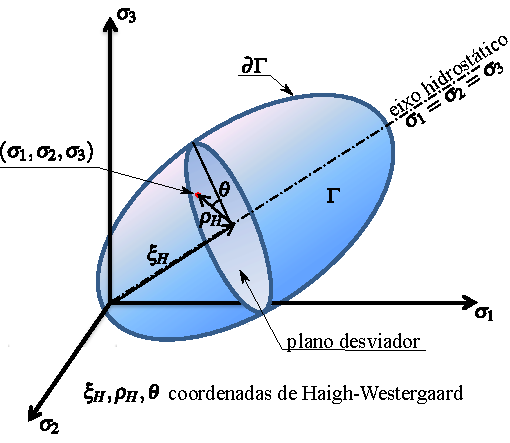
\includegraphics[scale = 1.0]{0504-dominio generico plasticamente admissivel.pdf}
	\end{center}
	\caption{\label{dominio_plasticamente_admissivel}Domínio genérico plasticamente admissível $\Gamma$ no espaço das tensões principais}
\end{figure}
Em elastoplasticidade isotrópica, a função de escoamento pode ser descrita apenas em função dos invariantes do tensor de tensões e das forças associadas às variáveis internas. São, portanto, comuns as seguintes representações equivalentes (adaptado de \citeauthor{Chen1988}, \citeyear{Chen1988}, p. 53-72):
\begin{equation}
	\label{eq:funcoes_escoamento}
	f(\sigmall,\ql) = f(I_1,J_2,J_3,\ql) = f(\xi_{H},\rho_{H},\theta,\ql) = f(p,q,\theta,\ql) = f(\sigma_{oct},\tau_{oct},\theta,\ql)
\end{equation}
em que:
\begin{equation}
	\label{eq:invariantes_tensores}
		\begin{array}{lcl}
			I_1 = \text{tr}(\sigmall) = \sigma_{11}+\sigma_{22}+\sigma_{33}\\
			J_2 = \dfrac{1}{2}\text{tr}(\sll^2) = \dfrac{1}{6}\left[ (\sigma_{11}-\sigma_{22})^2 + (\sigma_{22}-\sigma_{33})^2 + (\sigma_{33}-\sigma_{11})^2 \right] + \sigma_{12}^2+ \sigma_{23}^2+ \sigma_{13}^2, \\
			J_3 = \dfrac{1}{3}\text{tr}(\sll^3) = \text{det}(\sll) = s_{11}s_{22}s_{33}-s_{11}\sigma_{23}^2-s_{22}\sigma_{13}^2-s_{33}\sigma_{12}^2+2\sigma_{12}\sigma_{23}\sigma_{13}, \\ 
			\xi_{H} = p = \sigma_{oct} = \dfrac{1}{3}I_1, ~~~ \rho_{H} = \sqrt{\sll:\sll} = \sqrt{2J_2}, ~~~ \theta = \dfrac{1}{3}\text{asin}\left( \dfrac{-3\sqrt{3}}{2} \dfrac{J_3}{J_2^{3/2}} \right), \\
			-\dfrac{\pi}{6} \le \theta \le \dfrac{\pi}{6}, ~~~ q = \sqrt{\dfrac{3}{2}\sll:\sll} = \sqrt{3J_2}, ~~~ \tau_{oct} = \sqrt{\dfrac{3}{2}J_2},
	\end{array}
\end{equation}
sendo $(\xi_H,\rho_H,\theta)$ as coordenadas de Haigh-Westergaard (em que $\theta$ também é conhecido como ângulo de Lode), $p$ a pressão hidrostática, $q$ a tensão equivalente de von-Mises, $(\sigma_{oct},\tau_{oct})$ a tensão normal e cisalhante octaédrica, respectivamente, e $s_{ij}$ são as componentes do tensor de tensões desviadoras $\sll$, dado por:
\begin{equation}
	\label{eq:tensor_desviador}
	\sll = \sigmall: \left[ \Umllll-\Umll \otimes \Umll \right] = \sigmall - p\Umll.
\end{equation}

Quando a função de escoamento não depende de $I_1$   diz-se que a plasticidade é independente da pressão hidrostática, sendo determinada apenas pelo estado de tensões ao longo do plano desviador.

Diversas funções de escoamentos podem ser obtidas na literatura, tal como as apresentadas no resumo de \citeonline{Viladkar1995} que reúne tanto as funções de escoamentos clássicas (von-Mises, Tresca, Drucker-Prager, Mohr-Coulomb) quanto mais sofisticadas (\textit{Cap Models, Critical State Model, Desai’s Generlized Model}). O presente trabalho utilizará as funções de escoamentos de Drucker-Prager (DP) e Mohr-Coulomb (MC) que compreendem também generalizações das funções de von-Mises (VM) e Tresca (TR), respectivamente (\autoref{Funções_escoamento}).
\begin{figure}[H]
	\begin{center}
		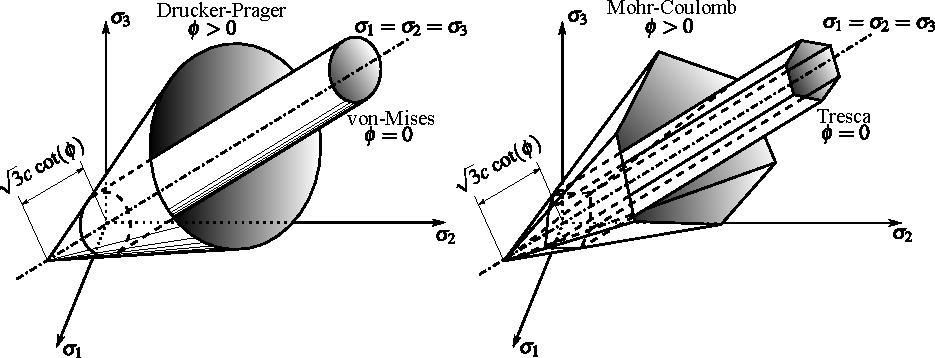
\includegraphics[scale = 1.0]{0505-funções de escoamento.pdf}
	\end{center}
	\caption{\label{Funções_escoamento}Funções de escoamento de a) Drucker-Prager e b) Mohr-Coulomb  (adaptado de: \citeonline[p. 824]{Zienkiewicz1974})}
\end{figure}
A função de escoamento de Mohr-Coulomb, representada através de invariantes, é dada por \cite[p. 166]{Neto2008}:
\begin{equation}
	\label{eq:f_Mohr_Coulomb}
	f(\sigmall,\ql) = f(I_1,J_2,\theta,c,\phi) = \dfrac{\sin(\phi)}{3}I_1 + \left(\cos(\theta)-\dfrac{1}{\sqrt{3}}\sin(\theta)\sin(\phi)\right)\sqrt{J_2}-c\cos(\phi) 
\end{equation}
em que $c$ é a coesão e $\phi$ o ângulo de atrito. De forma análoga, a função de escoamento de Drucker-Prager é dada por \cite[p. 167]{Neto2008}:
\begin{equation}
	\label{eq:f_Drucker_Prager}
	f(\sigmall,\ql) = f(I_1,J_2,\beta,k) = \beta I_1 +\sqrt{J_2}-k
\end{equation}
em que os parâmetros $\beta$ e $k$ podem ser relacionados com a coesão e o ângulo de atrito do modelo de Mohr-Coulomb. Para o caso em que a superfície de Drucker-Prager coincide com as bordas mais externas da superfície de Mohr-Coulomb tem-se \cite[p. 167]{Neto2008}:
\begin{equation}
	\label{eq:f_DP_bordasexternas_MC}
	\beta = \dfrac{2\sin{\phi}}{\sqrt{3}(3-\sin(\phi))}, ~~~ k = \dfrac{6\cos{\phi}}{\sqrt{3}(3-\sin(\phi))}c,
\end{equation}
e para o caso em que a superfície de Drucker-Prager coincide com as bordas mais internas da superfície de Mohr-Coulomb, tem-se \cite[p. 167]{Neto2008}:
\begin{equation}
	\label{eq:f_DP_bordasinternas_MC}
	\beta = \dfrac{2\sin{\phi}}{\sqrt{3}(3+\sin(\phi))}, ~~~ k = \dfrac{6\cos{\phi}}{\sqrt{3}(3+\sin(\phi))}c.
\end{equation}

Essa aproximação pode ser vista no plano desviador conforme a \autoref{DP-MC-plano_desviador}.
\begin{figure}[H]
	\begin{center}
		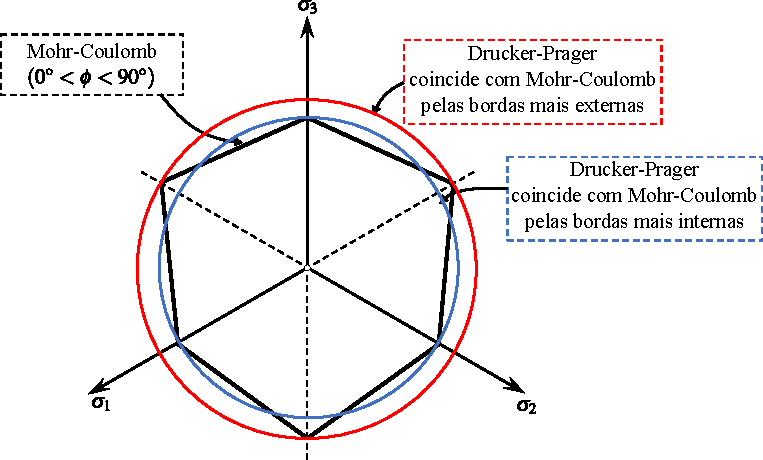
\includegraphics[scale = 1.0]{0506-representação no plano desviador da aproximação da superficie de MC com DP.pdf}
	\end{center}
	\caption{\label{DP-MC-plano_desviador}Representação no plano desviador da aproximação da superfície de Mohr-Coulomb pela superfície de Drucker-Prager  (adaptado de: \citeauthor{Neto2008}, \citeyear{Neto2008}, p. 169)}
\end{figure}
Quando $\phi = 0$ a superfície de Mohr-Coulomb e a de Drucker-Prager se tornam independentes da pressão hidrostática e se particularizam, respectivamente, para a superfície de Tresca e von-Mises (adaptado de: \citeauthor{Neto2008}, \citeyear{Neto2008}, p. 162-163):
\begin{equation}
	\label{eq:f_Tresca}
	f(\sigmall,\ql) = f(J_2,\theta,c) = \sqrt{J_2}\cos{\theta} - c,
\end{equation}
\begin{equation}
	\label{eq:f_von-Mises}
	f(\sigmall,\ql) = f(J_2,\theta,c) = \sqrt{3}\sqrt{J_2} - 2c.
\end{equation}

Igualando-se as expressões (\ref{eq:f_von-Mises}) e (\ref{eq:f_Tresca}) à zero e isolando $\sqrt{J_2}$ é possível relacionar ambas as superfícies através da coesão (\autoref{TR-VM-plano_desviador}):
\begin{equation}
	\label{eq:ctr_cvm}
	c_{\text{TR}} = \dfrac{2}{\sqrt{3}}\cos(\theta)c_{\text{VM}} = \left\{
	\begin{array}{lcl}
		\dfrac{2}{\sqrt{3}}c_{\text{VM}}, ~~~\text{se}~\theta = 0^\circ \\ 
		c_{\text{VM}},~~~~~~~~~\text{se}~\theta = 30^\circ
	\end{array}
	\right..
\end{equation}
\begin{figure}[H]
	\begin{center}
		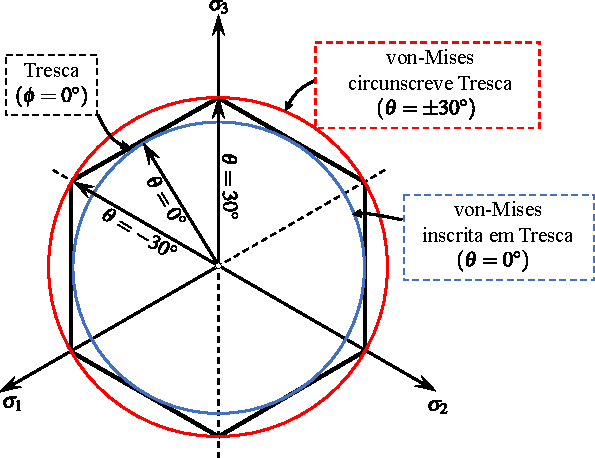
\includegraphics[scale = 1.0]{0507-representação no plano desviador da aproximação da superfície de TR e VM.pdf}
	\end{center}
	\caption{\label{TR-VM-plano_desviador}Representação no plano desviador da aproximação da superfície de Tresca pela superfície de von-Mises (adaptado de: \citeauthor{Neto2008}, \citeyear{Neto2008}, p. 159, 164)}
\end{figure}

\subsection{Regra de fluxo plástico}

A regra de fluxo plástico descreve a lei de evolução das deformações plásticas com relação às tensões. Essa regra é postulada da seguinte forma:
\begin{equation}
	\label{eq:fluxo_elastoplastico}
	\dot \varepsilonll^p = \dot \lambda \dgdsll
\end{equation}
em que $\dot \lambda$ é a taxa da magnitude de deformação plástica $\lambda$ (chamado também de multiplicador plástico) e $\dgdsll$ o tensor que dá a direção do fluxo plástico (conhecido também como vetor de fluxo ou gradiente do potencial plástico), sendo definido como:
\begin{equation}
	\label{eq:vetor_fluxo_elastoplastico}
	\dgdsll = \dfrac{\partial g}{\partial \sigmall}
\end{equation}
em que $g$ é uma função análoga a $f$ chamada de potencial plástico. No caso em que $g=f$ tem-se a \textbf{plasticidade associada} (ou seja, a direção do fluxo plástico é perpendicular à superfície de plastificação) (\autoref{fluxo_associado}).
\begin{figure}[H]
	\begin{center}
		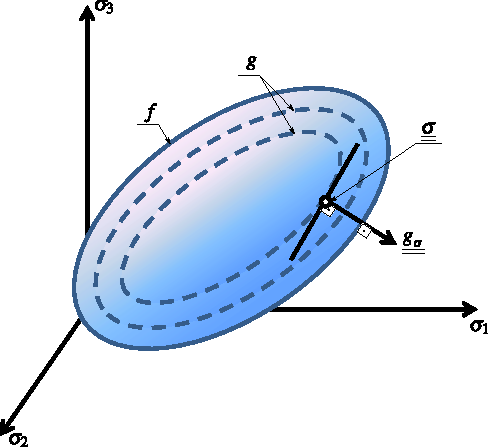
\includegraphics[scale = 1.0]{0508-representacao geometrica do vetor de fluxo com plasticidade associada.pdf}
	\end{center}
	\caption{\label{fluxo_associado}Representação geométrica do vetor de fluxo em plasticidade associada (adaptado de: \citeonline[p. 182]{Chen1988})}
\end{figure}
Tal como a função de escoamento, o potencial plástico geralmente é descrito através dos invariantes do tensor de tensões e seu gradiente pode ser determinado aplicando a regra da cadeia em (\ref{eq:vetor_fluxo_elastoplastico}). Por exemplo, se $g(I_1,\sqrt{J_2},J_3,\ql)$, tem-se (adaptado de \citeonline[p. 231]{Owen1980}):
\begin{equation}
	\label{eq:invariantes_tensores}
	\begin{array}{lcl}
		\dgdsll = C_1\gllum + C_2\glldois + C_3\glltres, \\ 
		\gllum = \dfrac{\partial I_1}{\partial \sigmall} = \Umll,~~~ \glldois = \dfrac{\partial \sqrt{J_2}}{\partial \sigmall} = \dfrac{1}{2\sqrt{J_2}}\sll,~~~ \glltres = \dfrac{\partial J_3}{\partial \sigmall}, \\
		C_1 = \dfrac{\partial g}{\partial I_1},~~~C_2=\dfrac{\partial g}{\partial \sqrt{J_2}}-\dfrac{\tan{(3\theta)}}{\sqrt{J_2}}\dfrac{\partial g}{\partial \theta},~~~C_3 = -\dfrac{\sqrt{3}}{2\cos{(3\theta})}\dfrac{1}{J_2^{3/2}}\dfrac{\partial g}{\partial \theta},
	\end{array}
\end{equation}
sendo que nessa descrição, apenas as constantes $C_1$, $C_2$  e $C_3$ são particularidades das diferentes superfícies potenciais, conforme \autoref{tab:c1c2c3}. 

\begin{table}[H]
	\caption{Constantes para o cálculo do gradiente do potencial plástico (adaptado de \citeonline[p. 231]{Owen1980}}
	\label{tab:c1c2c3}
	\centering
	\small
	\renewcommand{\arraystretch}{1.25}
	\begin{tabular}{c c c c}
		\hline
		\multicolumn{1}{c}{\textbf{SUPERFÍCIE}} &
		\multicolumn{1}{c}{{$\mathbf C_1$}} &
		\multicolumn{1}{c}{{$\mathbf C_2$}} &
		\multicolumn{1}{c}{{$\mathbf C_3$}} \\
		\hline
		TR & $0$ & $2\cos{\theta}(1+\tan{\theta}\tan{3\theta})$ & $\dfrac{\sqrt{3}}{J_2}\dfrac{\sin{\theta}}{\cos{3\theta}}$ \\		
		VM & $0$ & $\sqrt{3}$ & $0$ \\
		MC & $\dfrac{1}{3}\sin(\phi)$ &  $\scriptstyle \cos(\theta)\left[1 +\tan(\theta)\tan(3\theta)+\dfrac{\scriptstyle \sin(\phi)\left[\tan(3\theta)-\tan(\theta)\right]}{\scriptstyle \sqrt{3}}\right]$ & $\dfrac{\sqrt{3}\sin(\theta)+\cos(\theta)\sin(\phi)}{2J_2\cos(3\theta)}$ \\		
		DP & $\beta$ & $1$ & $0$ \\			
		\hline
	\end{tabular}
	\normalsize
\end{table}

Nas expressões de $C_2$ e $C_3$, pode-se ver que o vetor de fluxo de Mohr-Coulomb, e consequentemente o de Tresca, possui uma singularidade quando $\theta = \pm \pi/6$. Isso ocorre devido a essas superfícies apresentarem um vértice nessas coordenadas no plano desviador. Há diversas formas de se resolver esse problema, sendo que a adotada no presente trabalho, dada por \citeonline[p. 234]{Owen1980}, será utilizar os valores de $C_1$,$C_2$ e $C_3$ de Drucker-Prager (ou von-Mises) quando $\theta = \pm \pi/6$.

Um aspecto comum na geomecânica é a variação do volume do material durante a evolução das deformações plásticas. Esse efeito é comumente introduzido através da plasticidade não associada, adotando, ao invés do ângulo de atrito, um ângulo de dilatância $0<\psi<\phi$  na função potencial $g$.

\subsection{Lei de endurecimento/amolecimento}
A lei de endurecimento/amolecimento fornece a regra de evolução da superfície de escoamento ao longo das deformações plásticas (\textit{strain-hardening/softening}) ou do trabalho plástico (\textit{work-hardening/softening}). Para a presente tese, será adotado o primeiro caso e a lei é então postulada da seguinte forma \cite[p. 249]{Belytschko2000}:
\begin{equation}
	\label{eq:amolecimento}
	\dot \ql = \dot \lambda \hl = - \dot \lambda \dfrac{\partial h}{\partial \ql}
\end{equation}
em que $\hl = - \partial h / \partial \ql$ é um vetor que contém os gradientes de uma função potencial $h$ com relação às forças termodinâmicas associadas. Como a função de escoamento $f$ é dependente de $\ql$, a mudança dessas ao longo da deformação plástica irá alterar a posição e/ou a forma da superfície de escoamento. Quando a superfície de escoamento é estática, ou seja, $\dot \ql=\underline 0$, tem-se a plasticidade perfeita, quando esta aumenta tem-se o endurecimento isotrópico e quando se desloca tem-se o endurecimento cinemático, sendo mista, quando composta das duas últimas (\autoref{tipos_endurecimento}).

\begin{figure}[H]
	\begin{center}
		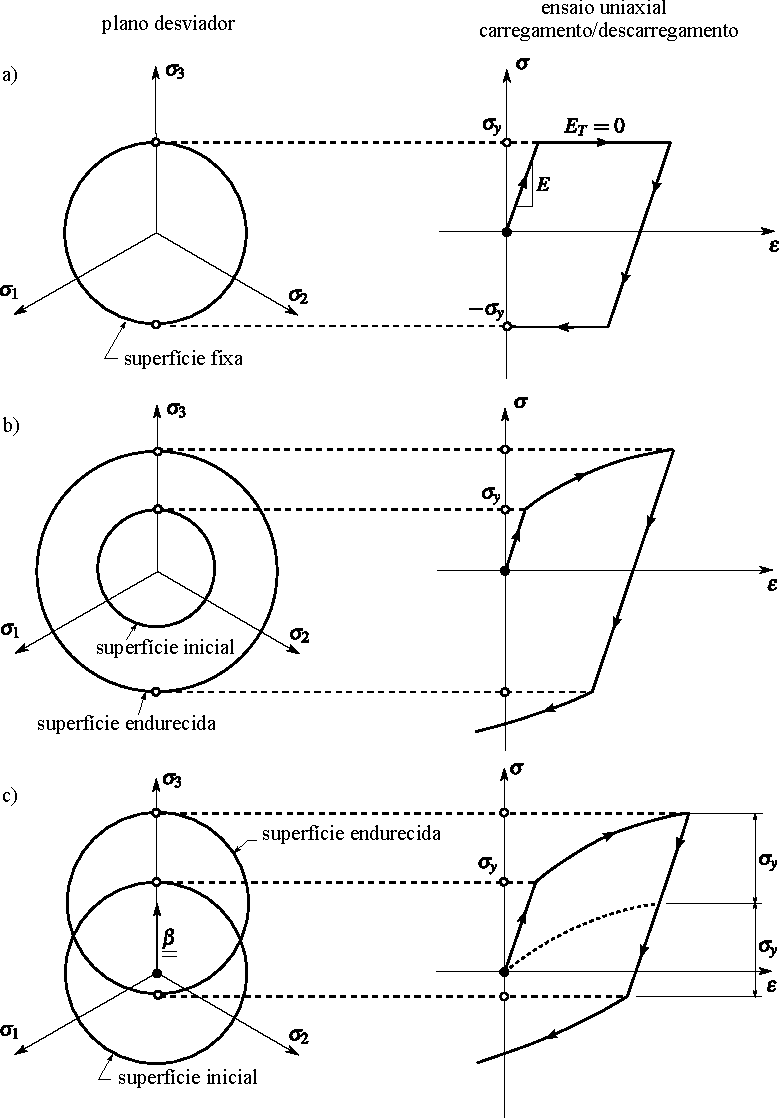
\includegraphics[scale = 1.0]{0509-tipos_endurecimentos.pdf}
	\end{center}
	\caption{\label{tipos_endurecimento}Representação dos tipos de endurecimento no plano desviador e na curva tensão-deformação: a) elastoplasticidade perfeita, b) endurecimento isotrópico e c) endurecimento cinemático (adaptado de: \citeauthor{Neto2008}, \citeyear{Neto2008}, p. 178, 179, 186)}
\end{figure}
Em um primeiro momento, no presente trabalho, não é considerado a influência da lei de endurecimento e as forças termodinâmicas serão constantes ao longo do histórico de deformações, ou seja, $\dot \ql = \underline 0$. Nesse caso, tem-se a elastoplasticidade perfeita. Em um segundo momento é considerado a lei de endurecimento/amolecimento associada ($h = f$) e isotrópica. Portanto, a força termodinâmica associada é dada exclusivamente pela parcela que não depende da parte hidrostática ($I_1$) e nem desviadora ($J_2$) nas superfícies de escoamento. Essa força será controlada pelo parâmetro coesivo, de modo que $q = \chi c(\bar \varepsilon^p)$ em que:
\begin{equation}
	\label{eq:dfdc}
	\chi = \left\{ \begin{array}{ll} 
		2, & \text{para von-Mises} \\
		\dfrac{6\cos{\phi}}{\sqrt{3}(3\pm \sin(\phi))}, & \text{para Drucker-Prager} \\ 
		1, & \text{para Tresca}\\
		\cos(\phi), & \text{para Mohr-Coulomb}\end{array}	
	\right.
\end{equation}



sendo a deformação plástica equivalente $\bar \epsilon^p$ a variável de estado. Para a coesão, é considerado uma função linear definida por partes, conforme \autoref{funcao_coesao}, de modo a representar o endurecimento/amolecimento característico do maciço, tal como vistos no Capítulo 4.3.
\begin{figure}[H]
	\begin{center}
		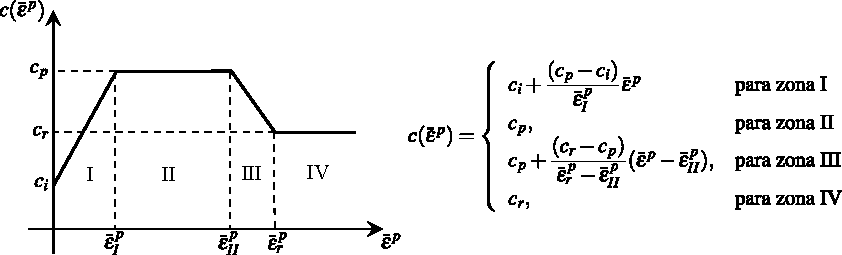
\includegraphics[scale = 1.0]{0510-lei de endurecimento ou amolecimento_coesao.pdf}
	\end{center}
	\caption{\label{funcao_coesao}Função linear definida por partes para representar o endurecimento/amolecimento através do parâmetro coesivo (adaptado de: \citeonline[p. 158]{Potts1999}}
\end{figure}
Portanto, usando a regra da cadeia, escreve-se (\ref{eq:amolecimento}) da seguinte forma:
\begin{equation}
	\label{eq:expressao_amolecimento}
	\dot q = - \dot \lambda \dfrac{\partial h}{\partial q} = - \dot \lambda \dfrac{\partial f}{\partial q} = \dot \lambda \left(- \dfrac{\partial f}{\partial q}\dfrac{\partial q}{\partial c}\dfrac{\partial c}{\partial \bar \epsilon^p}\right)	
\end{equation}
sendo, seus termos, conforme (\ref{eq:f_Mohr_Coulomb}), (\ref{eq:f_Drucker_Prager}), (\ref{eq:f_Tresca}), (\ref{eq:f_von-Mises}) e \autoref{funcao_coesao}, dados por:
\begin{equation}
	\label{eq:dfdq}
	\dfrac{\partial f}{\partial q} = -1,~\dfrac{\partial q}{\partial c} = \chi,
\end{equation}
e
\begin{equation}
	\label{eq:dqde}
	\dfrac{\partial c}{\partial \bar \epsilon_{p}} = \left\{ \begin{array}{ll} \dfrac{(c_p-c_i)}{\bar \epsilon^p_I} &  \text{para zona I} \\ 
	0, & \text{para zona II} \\
	\dfrac{(c_r-c_p)}{\bar \epsilon^p_{r}-\bar \epsilon^p_{II}}, & \text{para zona III} \\	
	0, & \text{para zona IV}
\end{array}\right..
\end{equation}

O valor da deformação plástica efetiva é calculada a partir da seguinte expressão:
\begin{equation}
	\label{eq:epsPeq}
	\dot{{\bar \epsilon}}^p = C||\dot \varepsilonll^p||
\end{equation}
em que
\begin{equation}
	\label{eq:epsPeq}
	||\dot \varepsilonll^p|| = \sqrt{(\dot{\varepsilon}^{p}_{11})^2 + (\dot{\varepsilon}^{p}_{22})^2 + (\dot{\varepsilon}^{p}_{33})^2 + 2(\dot{\varepsilon}^{p}_{12})^2 + 2(\dot{\varepsilon}^{p}_{23})^2 + 2(\dot{\varepsilon}^{p}_{13})^2}
\end{equation}

e $C$ a rigor depende da superfície de plasticidade, do gradiente do potencial plástico e do estado de tensões ao qual está submetido a amostra no ensaio. Sua dedução é feita através do trabalho plástico por unidade de volume. Para o presente trabalho, será utilizado a seguinte expressão deduzida para Drucker-Prager, que considera plasticidade associada e estados de tensões gerais (adaptado de \citeauthor{Chen1988}, \citeyear{Chen1988}, p. 257-259):
\begin{equation}
	\label{eq:Czao}
	C = \dfrac{\beta+1/\sqrt{3}}{\sqrt{3\beta^2+1/2}}.
\end{equation}
Quando $\phi = 0$ o material é independente da pressão hidrostática, ou seja, $\beta = 0$ e tem-se $C = \sqrt{2/3}$.

\subsection{Condições de carregamento e descarregamento}

A evolução das equações (\ref{eq:fluxo_elastoplastico}) e (\ref{eq:amolecimento}) estão sujeitas à três condições (condições de Kuhn-Tucker), que são (\citeauthor{Neto2008}, \citeyear{Neto2008}, p. 170):
\begin{equation}
	\label{eq:kuhntucker}
	f \le 0,~~~ \dot \lambda \ge 0, ~~~ \dot \lambda f = 0.
\end{equation}
Essas condições estabelecem que apenas ocorre fluxo plástico quando o estado de tensões está sobre a superfície de escoamento e, neste caso, não há variação da função de escoamento, ou seja:
\begin{equation}
	\label{eq:consistencia}
	\dot f = \dfrac{\partial f}{\partial \sigmall}:\dot \sigmall + \dfrac{\partial f}{\partial \ql}\cdot \dot \ql = \dfdsll:\dot \sigma + \dfdql \cdot \dot \ql = 0.
\end{equation}

A equação (\ref{eq:consistencia}) é conhecida como \textbf{condição de consistência}.

\subsection{Multiplicador plástico e módulo elastoplástico contínuo}
Introduzindo na condição de consistência (\ref{eq:consistencia}) a relação constitutiva (\ref{eq:leielastoplastica}), o fluxo plástico (\ref{eq:fluxo_elastoplastico}), a lei de endurecimento/amolecimento (\ref{eq:amolecimento}) e isolando o multiplicador plástico tem-se:
\begin{equation}
	\label{eq:lambda}
	\dot \lambda = \dfrac{\dfdsll:\Dllll:\dot \varepsilonll}{\dfdsll:\Dllll:\dgdsll-\dfdql \cdot \hl}
\end{equation}
que introduzindo na relação constitutiva (\ref{eq:leielastoplastica}) leva à:
\begin{equation}
	\label{eq:Dep}
	\Dllll^{ep} = \Dllll - \dfrac{\left(\Dllll:\dgdsll \right)\otimes\left(\dfdsll:\Dllll \right)}{\dfdsll:\Dllll:\dgdsll-\dfdql \cdot \hl}
\end{equation}
em que $\otimes$ é o produto tensorial. Através de (\ref{eq:Dep}) pode-se notar que se a plasticidade for associada o tensor constitutivo elastoplástico é simétrico. Também, pelo sinal do segundo termo, pode-se ver que a plasticidade representa uma redução no módulo de elasticidade do material.

\section{Modelo constitutivo viscoplástico}

\subsection{Decomposição do tensor de deformação total}
Considerando a hipótese das pequenas transformações é válida a decomposição do tensor de deformação total em uma componente elástica e outra viscoplástica, de modo que:
\begin{equation}
	\label{eq:decomposicao_deformacoes_vp}
	\dot \varepsilonll = \dot \varepsilonll^e + \dot \varepsilonll^{vp} 
\end{equation}
em que $\dot \varepsilonll^{vp}$ é conhecido como fluxo viscoplástico. No caso da viscoplasticidade, a lei constitutiva depende tanto do trajeto das tensões quanto do tempo (e por isso também conhecida como \textit{rate-dependent plasticity}), representando-se então as quantidades como taxas em um tempo real. Seguindo o mesmo raciocínio da elastoplasticidade, a relação constitutiva elastoviscoplástica linearizada pode ser escrita conforme:
\begin{equation}
	\label{eq:leielastoviscoplastica}
	\dot \sigmall = \Dllll^{vp}:\dot \varepsilonll = \Dllll:\dot \varepsilonll^e = \Dllll:\left(\dot \varepsilonll - \dot \varepsilonll^{vp} \right)
\end{equation}
em que $\Dllll^{vp}$ é o tensor de quarta ordem que representa o módulo elastoviscoplástico contínuo.

\subsection{Superfície de escoamento}

Em viscoplasticidade nem sempre se tem um regime elástico, por exemplo, a altas temperaturas certos materiais podem fluir sempre sobre tensão, ou seja, a função de escoamento é zero \cite[p. 448]{Neto2008}. Para esses casos, existem modelos como o de \citeonline{Norton1929}, \citeonline{Lemaitre1994}, e também funções provenientes de ajustes empíricos que descrevem o fluxo viscoplástico através da tensão, tempo e temperatura, como por exemplo, as resumidas por \citeonline{Skrzypek1993}. Porém, em geral, o comportamento viscoso do maciço em túneis evidencia-se após um determinado nível de tensões, conforme visto na \autoref{curva_caracteristica_fluencia_ensaio}. Para esses casos são adotadas superfícies de escoamento análogas as da elastoplasticidade. No presente trabalho serão utilizadas as mesmas superfícies do capítulo 5.5.2. Porém, ao contrário da elastoplasticidade, essa superfície não delimita um domínio plasticamente admissível podendo $f(\sigmall,\ql) > 0$.

\subsection{Regra de fluxo viscoplástico}
Tal como na elastoplasticidade, a regra de fluxo viscoplástico é postulada da seguinte forma:
\begin{equation}
	\label{eq:fluxo_viscoplastico}
	\dot \varepsilonll^{vp} = \dot \lambda \dgdsll
\end{equation}
em que $\dot \varepsilonll^{vp}$ é o fluxo viscoplástico (ou taxa de deformação viscoplástica), $\lambda$ a magnitude da deformação viscoplástica e $\dgdsll$ o vetor de fluxo viscoplástico, definido de forma igual ao da elastoplasticidade, ou seja, através do gradiente de uma função potencial $g$, porém viscoplástica.

\subsection{Lei de endurecimento/amolecimento}
Na viscoplasticidade o endurecimento pode ser incorporado fazendo com que as variáveis internas sejam função da magnitude da deformação viscoplástica acumulada:
\begin{equation}
	\label{eq:endurecimento_viscoplastico}
	\ql=\hl(\bar{\varepsilon}^{vp})
\end{equation}
em que
\begin{equation}
	\label{eq:epslonvpbar}
	\bar{\varepsilon}^{vp} = \int_{0}^{t}|\dot \lambda|dt.
\end{equation}

Contudo, no presente trabalho, apesar da generalidade dos algoritmos descritos na seção posterior, não será incorporado o endurecimento/amolecimento, se tratando, portanto, de uma viscoplasticidade perfeita.

\subsection{Multiplicador viscoplástico}
Como as deformações viscoplásticas ocorrem quando $f>0$ não há a imposição da condição de consistência. Dessa forma, tem-se que a taxa do multiplicador viscoplástico $\dot \lambda$ não pode ser obtida de uma condição do tipo $\dot f = 0$. Para contornar esse aspecto, existem modelos que fornecem uma expressão explícita para $\dot \lambda$, e no presente trabalho será adotado o modelo de Perzyna \cite[p. 823]{Zienkiewicz1974}:
\begin{equation}
	\label{eq:lambdavp}
	\dot \lambda = \dfrac{\Phi(f/f_0)}{\eta}
\end{equation}
\begin{equation}
	\label{eq:sobretensao}
	\Phi = \left\langle  \dfrac{f(\sigmall,\ql)}{f_0} \right\rangle^n
\end{equation}
em que $\eta$ é a constante de viscosidade dinâmica (unidade de tempo), $\Phi$ é a função de sobretensão, nesse caso, uma função potencial com expoente $n$, $f_0$ parâmetro de tensão convenientemente adotado a partir do qual se inicia o fenômeno viscoso e $\left\langle * \right\rangle$ é a função de McCauley, que é nulo quando $*<0$, ou seja, apenas ocorrerá fluxo viscoplástico quando o critério $f/f_0$ for positivo. O valor de $f_0$ a rigor depende da superfície viscoplástica adotada, conforme (adaptado de \citeonline[p. 239, 273]{Owen1980}:

\begin{equation}
	\label{eq:f0}
	f_0 = \left\{ \begin{array}{ll} 
		c, & \text{para Tresca} \\
		2c, & \text{para von-Mises} \\
		c\cos(\phi), & \text{para Mohr-Coulomb} \\ 
		 k, & \text{para Drucker-Prager}\end{array}	
	\right.
\end{equation}


Muitas vezes o parâmetro $f_0$ não consta na expressão como, por exemplo, em \citeonline[p. 222]{Rousset1988}. Nesse caso, seu valor está implícito na constante $\eta$ que possuí unidade de tempo vezes tensão elevada na potência $n$, ao invés de apenas a unidade de tempo, como em \citeonline{Zienkiewicz1974}. Isso não constitui um problema, pois, é mantida a consistência dimensional da expressão. Contudo, essa sutileza é importante no momento de adimensionalizar resultados com a expressão (\ref{eq:parametros_admensionais_vp}) da velocidade. Nessa expressão, \citeonline{Bernaud1991} utiliza a constante de viscosidade dinâmica conforme \citeonline{Rousset1988}.

\section{Modelo constitutivo elastoplástico viscoplástico}
O modelo elastoplástico-viscoplástico proposto nessa tese, dentro das hipóteses de pequenas transformações, compreende justamente a associação em série dos modelos constitutivos acima, portanto:
\begin{equation}
	\label{eq:decomposicao_deformacoes_epvp}
	\dot \varepsilonll = \dot \varepsilonll^e + \dot \varepsilonll^{p} + \dot \varepsilonll^{vp}.
\end{equation}

Essa associação pode ser vista na representação reológica da \autoref{modelo_reologico}.
\begin{figure}[H]
	\begin{center}
		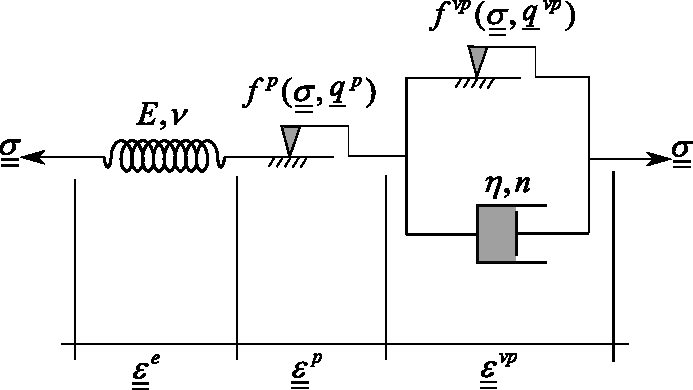
\includegraphics[scale = 1.0]{0510-representação reológica.pdf}
	\end{center}
	\caption{\label{modelo_reologico}Representação reológica do modelo elastoplástico-viscoplástico (adaptado de: \citeonline[p. 220]{Rousset1988})}
\end{figure}
Dessa forma, dentro das mesmas hipóteses dos modelos anteriores, a relação constitutiva linearizada fica sendo:
\begin{equation}
	\label{eq:lei_epvp}
	\dot \sigmall = \Dllll^{epvp}:\dot \varepsilonll = \Dllll:\dot \varepsilonll^e = \Dllll:\left(\dot \varepsilonll - \dot \varepsilonll^{p} - \dot \varepsilonll^{vp} \right).
\end{equation}

Uma observação importante é que as superfícies de escoamentos e as variáveis internas que definem a parcela elastoplástica e viscoplástica desse modelo podem ser diferentes entre si, incluindo a associação das suas respectivas funções potenciais com suas superfícies de escoamento. Apesar dessa abordagem genérica, na presente tese será adotada inicialmente a proposta seguida pelas soluções analíticas de \citeonline{Rousset1988} em que as forças termodinâmicas associadas às variáveis internas que governam a lei de endurecimento/amolecimento instantâneas e diferidas $\ql^p$ e $\ql^{vp}$, respectivamente, são funções multilineares de parâmetros coesivos em função da deformação plástica e viscoplástica equivalentes. Por exemplo para ilustrar esse comportamento, de forma unidimensional, segue-se as seguintes expressões \cite[p. 220]{Rousset1988}:
\begin{equation}
	\label{eq:qp_rousset}
	c(\varepsilon^p) = \left\{
		\begin{array}{lcl}
			2c - \dfrac{2(c-c_0)}{\varepsilon_0}\varepsilon^p \\ 
			2c_0~~~\text{se}~~~\varepsilon^p > \varepsilon_0
		\end{array}
	\right.
\end{equation}
que podem ser vistas graficamente na \autoref{lei_endurecimento_rousset}.
\begin{figure}[H]
	\begin{center}
		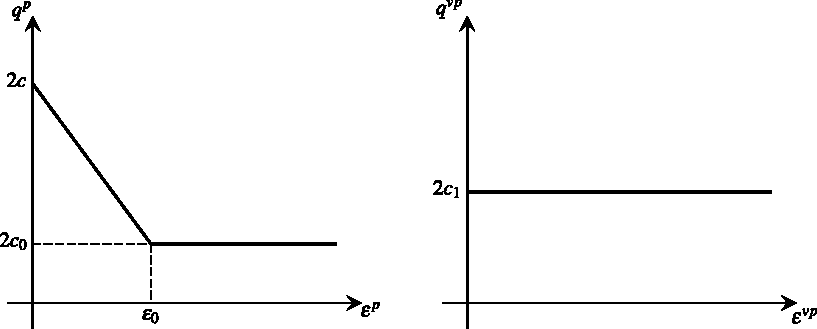
\includegraphics[scale = 1.0]{0511-lei de endurecimento ou amolecimento.pdf}
	\end{center}
	\caption{\label{lei_endurecimento_rousset}Leis de endurecimento e amolecimento para a parcela elastoplástica (à esquerda) e viscoplástica (à direita) (adaptado de: \citeonline[p. 220]{Rousset1988})}
\end{figure}
Nesse modelo, pode-se notar que a elastoplasticidade possui um amolecimento bilinear e a viscoplasticidade é perfeita. Os valores das coesões possuem a seguinte relação entre si: $c_0 < c_1 < c$. Essa relação não é arbitrária e pretende representar o inicio do comportamento diferido frente ao comportamento instantâneo. Essa desigualdade implica que as deformações viscoplásticas tenham inicio antes mesmo do maciço atingir sua resistência máxima de curto prazo e se mantém mesmo após o maciço ter atingido sua coesão residual. Generalizando para o caso tridimensional, para um determinado ponto no interior do maciço, tem-se, para seu estado de tensões, os domínios apresentados na \autoref{dominios_debernardi}.
\begin{figure}[H]
	\begin{center}
		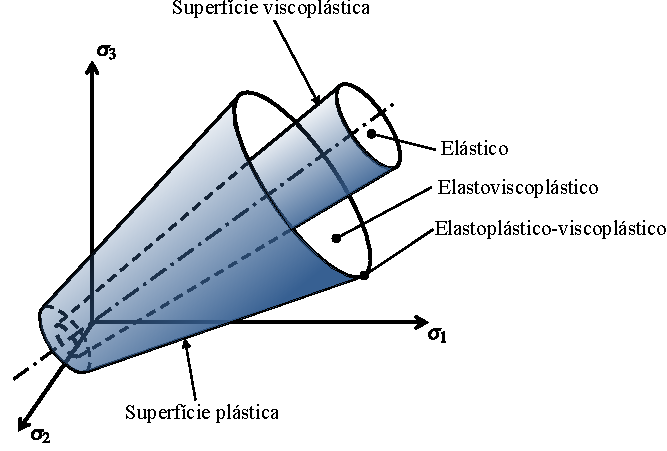
\includegraphics[scale = 1.0]{0512-dominios_superficie_epvp.pdf}
	\end{center}
	\caption{\label{dominios_debernardi}Domínios e superfícies do modelo elastoplástico-viscoplástico (adaptado de: \citeonline[p. 263]{Debernardi2009})}
\end{figure}
O comportamento desse modelo reológico pode ainda ser melhor entendido através da resposta das tensões frente a uma taxa de deformação constante. Esse comportamento é ilustrado na \autoref{resposta_epvp_deformacao_constante}, sendo $\dot \varepsilon_1 = \infty > \dot \varepsilon_2 > \dot \varepsilon_3 > \dot \varepsilon_4 = 0$.
\begin{figure}[H]
	\begin{center}
		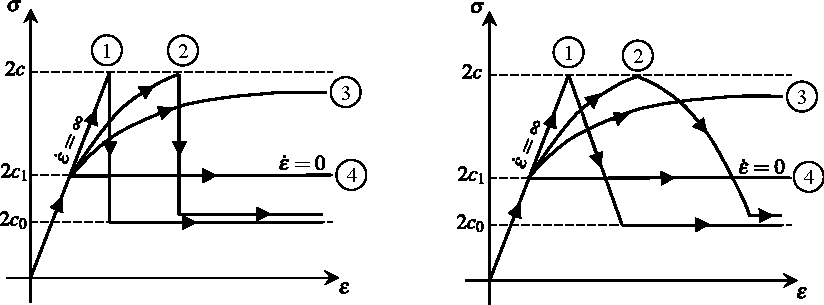
\includegraphics[scale = 1.0]{0513-resposta_epvp_deformacao_constante.pdf}
	\end{center}
	\caption{\label{resposta_epvp_deformacao_constante}Resposta do sistema a uma solicitação $\dot \varepsilon = \text{const}$ (adaptado de: \citeonline[p. 221]{Rousset1988})}
\end{figure}
Para altas taxas de deformação (caso 1 e 2), a tensão aumenta rapidamente até atingir o valor limite de $2c$ e em seguida diminui abruptamente (ruptura frágil) ou gradualmente (ruptura dúctil) mantendo uma tensão residual de $2c_0$. Pode-se notar que no caso 1, quando a taxa de deformação é muito alta, ao contrário do caso 2, os efeitos viscosos praticamente não ocorrem, tendo apenas o comportamento elastoplástico. Contudo, para taxas menores de deformação (caso 3) o limiar de ruptura não é atingido e a tensão evolui assintoticamente para um valor intermediário entre $2c$ e $2c_1$. Pode-se notar que no caso 4, quando a taxa de deformação é muito lenta, o modelo possui uma resposta elastoplástica perfeita com o limiar em $2c_1$.

%\section{Modelo constitutivo viscoelástico para o revestimento}

%Existem várias formulações para a previsão da deformação por fluência e retração do concretos disponíveis na literatura e nos códigos de projetos. Grade parte dessas formulações vêm de ajustes com dados experimentais e, como as características dos materiais são em grande parte condicionadas à região do ensaio, há uma certa aproximação devido a dispersão dos dados, com coeficientes de variação de 25,9\% à 67,4\%, dependendo da formulação como demonstrado por Fanourakis \& Ballim (2003). Nessa tese é utilizado o modelo desenvolvido por Dias (2013, et al. 2015) e ajustado e aplicado em problemas de túneis por Quevedo (2017). Esse modelo considera as formulações empíricas do Comité Euro-International du Béton (CEB-FIP Model Code 1990 ou CEB-MC90) com a fluência ajustada à teoria da solidificação de Bazant \& Prasannan (1989a,1989b). Esse ajuste é possível, pois, assim como na formulação de Bazant \& Prasannan, a formulação do CEB-MC90 separa o fator do coeficiente de fluência que depende do envelhecimento (idade do concreto) do fator de fluência que depende do tempo de aplicação da carga (idade da carga). Em vista dessa decomposição, a formulação e algoritmo apresentado por Bazant \& Prasannan permite modelar eficientemente os casos em que há um histórico de tensões variáveis, utilizando um modelo reológico de Kelvin-Generalizado para os parâmetros independnetes da idade do concreto.
